\chapter{Afprøvning}
\label{chapter:afproevning}

\section{Automatiserede tests}

I kraft af separationen mellem datamodeller og præsentationen samt håndteringen af disse, har vi valgt at implementere en række automatiserede tests udelukkende af datamodellerne.

Der er i samtlige tests, som involverer interaktion med en database, testet direkte mod de af Donkey understøttede databasesystemer. For at undgå utilsigtet indflydelse af tilstanden af testtabellerne, bliver disse derfor enten slettede eller tømt førend hver test. Ønskes testene kørt lokalt, gør vi derfor også opmærksomme på, at fungerende installationer af MySQL samt PostgreSQL er et krav. Disse skal ydermere være opsat med følgende databaser og tilhørende brugere (sans kodeord):

\begin{itemize}
  \item MySQL: \textbf{Database}: test, \textbf{bruger}: travis
  \item PostgreSQL: \textbf{Database}: test, \textbf{bruger}: postgres
\end{itemize}

\subsection{Kodedækning}
\label{subsection:kodedeakning}

\textit{Code coverage}-rapporter er blevet benyttede til at sikre en systematisk tilgang til implementation af tests. Disse rapporter er generede via kodedækningsredskabet JaCoCo\footnote{\url{https://github.com/jacoco/jacoco}} (se figur \ref{code-coverage:donkey}) og giver overblik over præcist hvilke instruktioner og eksekveringsgrene, der er berørte af de underliggende tests (\cite{wiki:code-cov}).

\begin{figure}[h]
  \begin{minipage}[b]{0.45\linewidth}
    \centering
    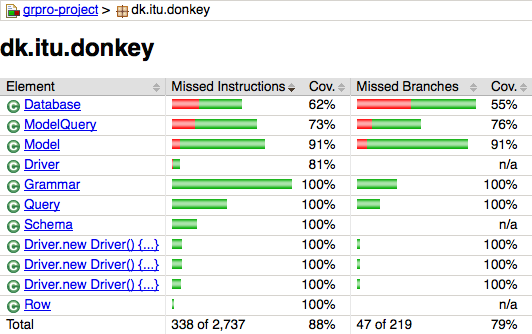
\includegraphics[width=\textwidth]{jacoco-donkey.png}
  \end{minipage}
  \hspace{0.5cm}
  \begin{minipage}[b]{0.45\linewidth}
    \centering
    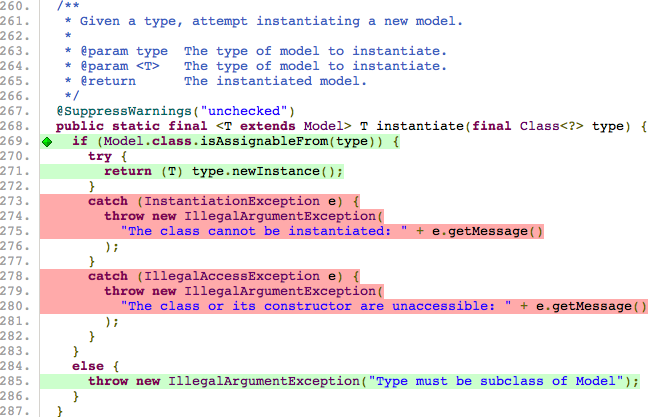
\includegraphics[width=\textwidth]{jacoco-model.png}
  \end{minipage}
  
  \caption{To udsnit af en JaCoCo kodedækningsrapport}
  \label{code-coverage:donkey}
\end{figure}

Vi har tilstræbet en dækningsprocent på minimum 80\% gennem vores testning af databaseabstraktionen under antagelse af, at de sidste 20\% overvejende er ikke- eller svært-testbar kode.

Da kodedækningsrapporten er et sæt af genererede HTML-sider, er disse ikke medtagede som bilag, men kan istedet frit tilgåes via følgende webadresse: \url{http://kasperisager.github.io/bookie/coverage}.

Det bør nævnes, at kodedækningsrapporter ikke nødvendigvis er en fuldstændig vandtæt løsning, da de udelukkende kan udtale sig om den tilsigtede eksekvering af den kode, som måtte være under test. En metode kan derfor i dækningsrapporten fremgå som værende fuldt dækket uden nødvendigvis at fungere under alle tænkelige forhold.

\subsection{Analyse af resultat}

Samtlige klasser i databaseabstraktionen er som nævnt ovenfor forsøgt minimum 80\% dækkede med tests. En oversigt over de forskellige tests kan findes på adressen \url{http://kasperisager.github.io/bookie/tests}, mens testene i deres fulde format kan findes i bilag \ref{appendix:tests}.

Med udgangspunkt i kodedækningsrapporten kan vi med stor sikkerhed konkludere, at vores databaseabstraktion virker efter hensigten under de forhold, som den er blevet benyttet i reservationssystemet.

\section{Brugerafprøvning}

Mens systematisk automatiseret testning af reservationssystemets JavaFX-baserede brugergrænseflade endnu er en mangelvare, vil vi lade brugervejledningen stå som brugerafprøvning. Den beskrevne funktionalitet i vejledningen er dermed den tilsigtede måde hvorpå reservationsystemets brugergrænseflade fungerer.

\subsection{Udestående fejl}

Som følge af brugerafprøvningen kan nævnes følgende fejl, som systemet endnu indeholder:

\begin{itemize}
  \item Vælges sæder (figur \ref{screenshot:chosen-seats}) og gåes der herefter til \textit{Reservationer}-fanen (figur \ref{screenshot:all-reservations}) hvorefter en reservation slettes (figur \ref{screenshot:delete-button}), vil de tidligere valgte sæder i længere være valgte, når der igen navigeres tilbage til \textit{Forestillinger}-fanen (figur \ref{screenshot:bookie}). Dette skyldes, er der efter sletning af en reservation foretages en genindlæsning af den valgte forestilling, således eventuelt nye reservationer bliver synlige.
\end{itemize}
